\section{eo\-Elitism$<$ EOT $>$ Class Template Reference}
\label{classeo_elitism}\index{eoElitism@{eoElitism}}
Straightforward elitism class, specify the number of individuals to copy into new geneneration or the rate w.r.t.  


{\tt \#include $<$eo\-Merge.h$>$}

Inheritance diagram for eo\-Elitism$<$ EOT $>$::\begin{figure}[H]
\begin{center}
\leavevmode
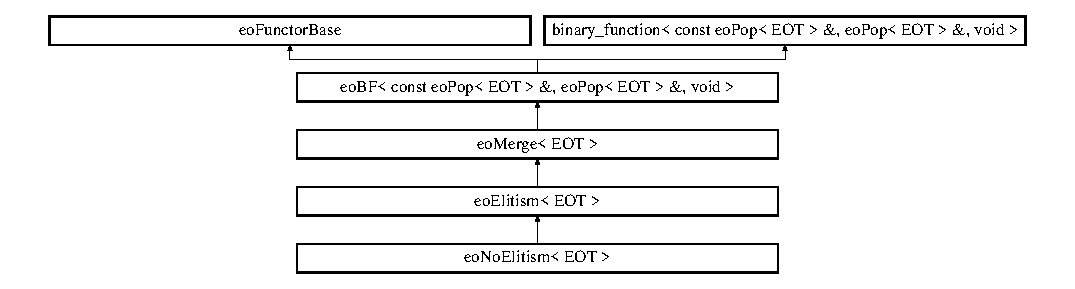
\includegraphics[height=3.4398cm]{classeo_elitism}
\end{center}
\end{figure}
\subsection*{Public Member Functions}
\begin{CompactItemize}
\item 
{\bf eo\-Elitism} (double \_\-rate, bool \_\-interpret\_\-as\_\-rate=true)\label{classeo_elitism_a0}

\item 
void {\bf operator()} (const {\bf eo\-Pop}$<$ {\bf EOT} $>$ \&\_\-pop, {\bf eo\-Pop}$<$ {\bf EOT} $>$ \&\_\-offspring)\label{classeo_elitism_a1}

\begin{CompactList}\small\item\em The pure virtual function that needs to be implemented by the subclass. \item\end{CompactList}\end{CompactItemize}
\subsection*{Private Attributes}
\begin{CompactItemize}
\item 
double {\bf rate}\label{classeo_elitism_r0}

\item 
unsigned {\bf combien}\label{classeo_elitism_r1}

\end{CompactItemize}


\subsection{Detailed Description}
\subsubsection*{template$<$class EOT$>$ class eo\-Elitism$<$ EOT $>$}

Straightforward elitism class, specify the number of individuals to copy into new geneneration or the rate w.r.t. 

pop size 



Definition at line 55 of file eo\-Merge.h.

The documentation for this class was generated from the following file:\begin{CompactItemize}
\item 
eo\-Merge.h\end{CompactItemize}
